%!TEX ROOT = thesis.tex
\chapter{THEORETICAL FRAMEWORK}
\label{chap: 3}

In this chapter we would start with a brief history of artificial intelligence research that are directly or indirectly related to the innovation of transformers. Then, the second section would covers the foundations of deep learning which includes feed-forward neural networks, activation functions, loss functions and evaluation metric. The third and final section would cover the basics of transformers.

\section{A Brief History of Deep Learning}

refer uday kamath


In the early 1940s, S. McCulloch and W. Pitts, using a simple electri-
cal circuit called a “threshold logic unit”, simulated intelligent behavior
by emulating how the brain works [179]. The simple model had the
first neuron with inputs and outputs that would generate an output 0
when the “weighted sum” was below a threshold and 1 otherwise, which
later became the basis of all the neural architectures. The weights were
not learned but adjusted. In his book The Organization of Behaviour
(1949), Donald Hebb laid the foundation of complex neural processing by proposing how neural pathways can have multiple neurons firing and
strengthening over time [108]. Frank Rosenblatt, in his seminal work,
extended the McCulloch–Pitts neuron, referring to it as the “Mark I
Perceptron”; given the inputs, it generated outputs using linear thresh-
olding logic [212].

The weights in the perceptron were “learned” by repeatedly passing
the inputs and reducing the difference between the predicted output
and the desired output, thus giving birth to the basic neural learning
algorithm. Marvin Minsky and Seymour Papert later published the book
Perceptrons which revealed the limitations of perceptrons in learning the
simple exclusive-or function (XOR) and thus prompting the so-called
The First AI Winter [186].

John Hopfield introduced “Hopfield Networks”, one of the first recur-
rent neural networks (RNNs) that serve as a content-addressable memory
system [117].

In 1986, David Rumelhart, Geoff Hinton, and Ronald Williams pub-
lished the seminal work “Learning representations by back-propagating
errors” [217]. Their work confirms how a multi-layered neural network
using many “hidden” layers can overcome the weakness of perceptrons
in learning complex patterns with relatively simple training procedures.
The building blocks for this work had been laid down by various research
over the years by S. Linnainmaa, P. Werbos, K. Fukushima, D. Parker,
and Y. LeCun [164, 267, 91, 196, 149].

LeCun et al., through their research and implementation, led to the
first widespread application of neural networks to recognize the hand-
written digits used by the U.S. Postal Service [150]. This work is a critical
milestone in deep learning history, proving the utility of convolution op-
erations and weight sharing in learning the features in computer vision.

Backpropagation, the key optimization technique, encountered a
number of issues such as vanishing gradients, exploding gradients, and
the inability to learn long-term information, to name a few [115].
Hochreiter and Schmidhuber, in their work,“Long short-term memory
(LSTM)” architecture, demonstrated how issues with long-term depen-
dencies could overcome shortcomings of backpropagation over time [116].

Hinton et al. published a breakthrough paper in 2006 titled “A fast
learning algorithm for deep belief nets”; it was one of the reasons for the
resurgence of deep learning [113]. The research highlighted the effective-
ness of layer-by-layer training using unsupervised methods followed by
supervised “fine-tuning” to achieve state-of-the-art results in character
recognition. Bengio et al., in their seminal work following this, offered deep insights into why deep learning networks with multiple layers can
hierarchically learn features as compared to shallow neural networks [27].
In their research, Bengio and LeCun emphasized the advantages of deep
learning through architectures such as convolutional neural networks
(CNNs), restricted Boltzmann machines (RBMs), and deep belief net-
works (DBNs), and through techniques such as unsupervised pre-training
with fine-tuning, thus inspiring the next wave of deep learning [28]. Fei-
Fei Li, head of the artificial intelligence lab at Stanford University, along
with other researchers, launched ImageNet, which resulted in the most
extensive collection of images and, for the first time, highlighted the
usefulness of data in learning essential tasks such as object recognition,
classification, and clustering [70]. Improvements in computer hardware,
primarily through GPUs, increasing the throughput by almost 10× ev-
ery five years, and the existence of a large amount of data to learn from
resulted in a paradigm shift in the field. Instead of hand-engineered fea-
tures that were the primary focus for many sophisticated applications,
by learning from a large volume of training data, where the necessary
features emerge, the deep learning network became the foundation for
many state-of-the-art techniques.

Mikolov et al. and Graves proposed language models using RNNs
and long short-term memory, which later became the building blocks for
many natural language processing (NLP) architectures [184, 97]. The
research paper by Collobert and Weston was instrumental in demon-
strating many concepts such as pre-trained word embeddings, CNNs for
text, and sharing of the embedding matrix for multi-task learning [60].
Mikolov et al. further improved the efficiency of training the word embed-
dings proposed by Bengio et al. by eliminating the hidden layer and for-
mulating an approximate objective for learning giving rise to “word2vec”,
an efficient large-scale implementation of word embeddings [185, 183].
Sutskever’s research, which proposed a Hessian-free optimizer to train
RNNs efficiently on long-term dependencies, was a breakthrough in re-
viving the usage of RNNs, especially in NLP [237]. Sutskever et al. in-
troduced sequence-to-sequence learning as a generic neural framework
comprised of an encoder neural network processing inputs as a sequence
and a decoder neural network predicting the outputs based on the in-
put sequence states and the current output states [238]. As a result, the
sequence-to-sequence framework became the core architecture for a wide
range of NLP tasks such as constituency parsing, named entity recogni-
tion (NER), machine translation, question-answering, and summariza-
tion, to name a few. Furthermore, even Google started replacing its monolithic phrase-based machine translation models with sequence-to-
sequence neural machine translation models [272]. To overcome the bot-
tleneck issues with the sequence-to-sequence framework, seminal work
by Bahdanau et al. proposed the attention mechanism, which plays a
crucial role in transformers and their variants [17].

\begin{figure}[ht]
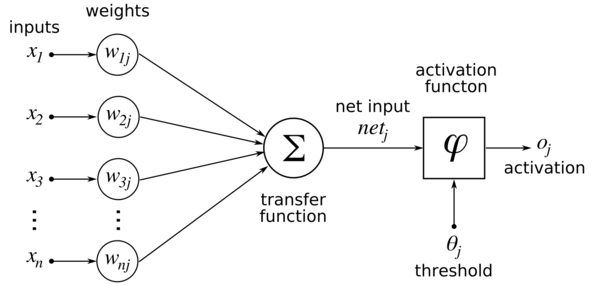
\includegraphics[width=10.5cm, height=5.5cm]{images/Rosenblattperceptron.png}
\centering
\caption{Rosenblatt Perceptron}
\label{fig:resenblatt-perceptron}
\end{figure}

\section{Theoretical Introduction to Deep Learning}
\subsection{Convolutional Neural Networks and Its Application in Semantic Segmentation of Satellite Images}

U-net, semua CNN jadah masuk sini.
\subsubsection{Activation Functions}
Sigmoid, RELU, softmax

\section{Introduction to Transformers}\label{subsection:Intro to Trans}
\subsection{Encoder-Decoder Architecture}
\subsection{Sequence-To-Sequence}
\subsection{Attention Mechanism}
\subsection{Embedding and Positional Encoding}
\subsection{sdsds}\label{sasas}
\section{Transformers Architecture}
%%%%%%%%%%%%%%%%%%%%%%%%%%%%%  ViT
\subsection{Vision Transformer (ViT)}
Vision Transformer from \cite{16x16} is the first group of researchers that experimented with Vision Transformer by applying a standard Transformer directly to images, with the fewest possible modifications. Their model is known as Vision Transformer (ViT) as it is the first Vision Transformer. They split an image into patches and provide the sequence of linear embeddings of these patches as an input to a Transformer. The image patches were treated the same way as word tokens do in an NLP application. This methods fails to capture the  translation equivariance and locality provide by the CNNs hence it is unsuitable for semantic segmentation task.

Another issue with Vision Transformer is the attention mechanism itself is $O(n^2)$ because it is a dot product thus requiring it to consume significant computational time and memory to capture the global context, which in turn, reducing its efficiency, scaling potential and its potential for real-world applications. Figure \ref{fig:vit} shows the ViT architecture.

\begin{figure}[ht]
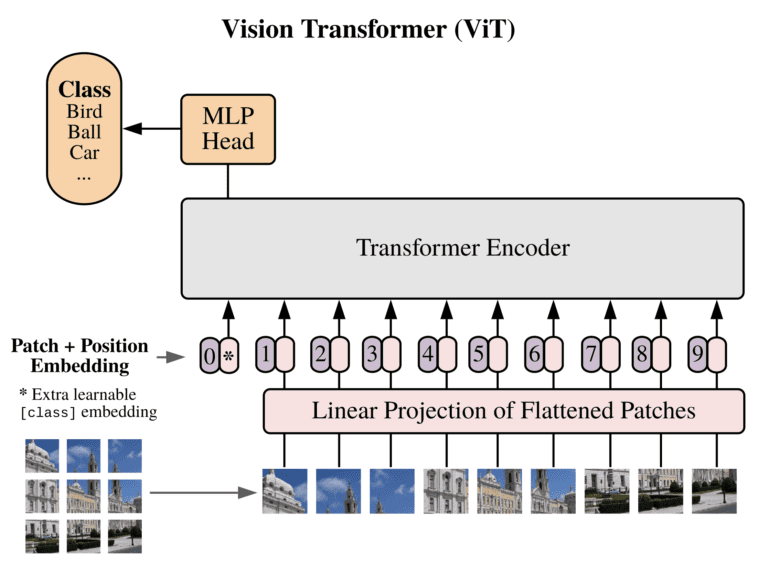
\includegraphics[width=13.5cm, height=9cm]{images/vision transformer.png}
\centering
\caption{ViT Architecture}
\label{fig:vit}
\end{figure}

%%%%%%%%%%%%%%%%%%%%%%%%%%%%%  Swin V1 and V2
\subsection{Swin Transformer}
The first version of Swin Transformer \cite{swin-v1} presents a hierarchical feature representation scheme that demonstrates impressive performances with linear computational complexity, which makes it suitable for semantic segmentation. The detailed mechanism of Transformers and Vision Transformers are discussed in chapter \ref{chap: 3}.

\FloatBarrier
\begin{figure}[ht]
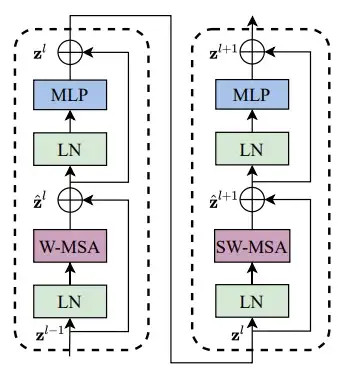
\includegraphics[width=9.5cm, height=7cm]{images/swin-architecture.jpg}
\centering
\caption{Swin Transformer V1 Architecture}
\label{fig:swin architecture}
\end{figure}

\begin{figure}[ht]
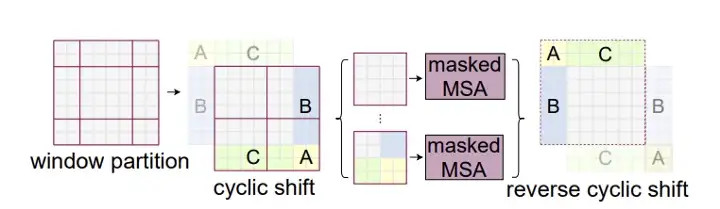
\includegraphics[width=13.5cm, height=5.5cm]{images/swin-cyclic-shift.jpg}
\centering
\caption{Cyclic Shifted Windows in Swin Transformer}
\label{fig:swin cyclic}
\end{figure}

\FloatBarrier
\begin{figure}[ht]
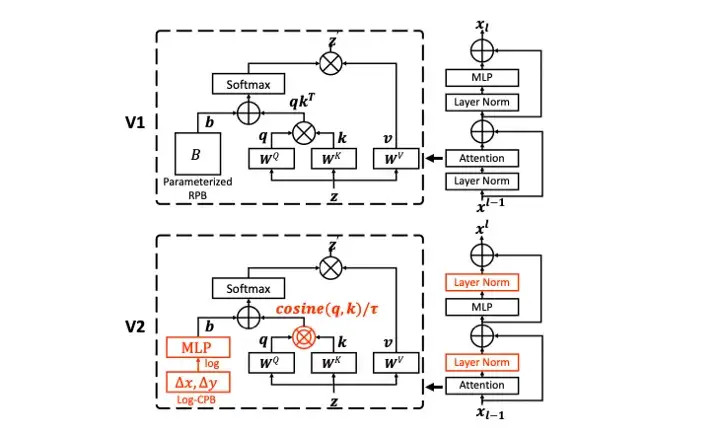
\includegraphics[width=13.5cm, height=9.5cm]{images/swin1-vs-swin2.jpg}
\centering
\caption{Difference Between Swin V1 and Swin V2}
\label{fig:swin v1 vs v2}
\end{figure}
\FloatBarrier

%%%%%%%%%%%%%%%%%%%%%%%%%%%%%  SegFormer
\subsection{SegFormer}

%%%%%%%%%%%%%%%%%%%%%%%%%%%%%  MaskFormer
\subsection{MaskFormer}

%%%%%%%%%%%%%%%%%%%%%%%%%%%% Beit
\subsection{Beit}

%%%%%%%%%%%%%%%%%%%%%%%%%%%%% DeeepLabV3
\subsection{DeepLabV3}
\section{Evaluation Metrics}
\section{Limitations}
\begin{enumerate}
    \item Imbalance class distribution.
    \item Inadequate computing.
    \item Quadratic computation complexity of the attention mechanism.
\end{enumerate}
